\chapter{Projekt Portfolio Management}

\section{Was verstehen wir unter (IT) Projekt Portfolio Management (PPM)?}

PPM legt systematisch und nachvollziehbar fest, welche Projekte in einem Planungszeitraum durchgeführt werden. Diese Projekte sollen die Unternehmensziele unterstützen und zusätzlich folgenden Kriterien gerecht werden:
\begin{itemize}
	\item Wirtschaftlichkeit (ROI)
	\item Beitrag zur Unternehmens- und IT-Strategie
	\item Projektrisiko (Realisierungswahrscheinlichkeit)
	\item Dringlichkeit
	\item Sicherheitsrelevanz
	\item Risikobereitschaft des Unternehmens
\end{itemize}

\section{Welche wesentlichen Aufgaben umfasst der PPM Prozess?}

\begin{enumerate}
	\item Bestandsaufnahme Projekte 
	\item Erfassung von Projektvorschlägen
	\item Bewertung der Vorschläge u.a. auf Basis Kosten, Nutzen, Risiko
	\item Portfolio-gestützte Auswahl anhand der definierten Kriterien
	\item Kommunikation der Entscheidungen
	\item Portfolio-Steuerung durch Projektcontrolling
\end{enumerate}

\section{Welche wesentlichen Gruppen von IT Aktiven können wir unterscheiden und wie verteilen sich die Investitionen auf diese?}

Es werden 4 Gruppen von IT Aktiven unterschieden. Die Prozentangabe ist der Anteil an den IT-Kosten in einem Unternehmen.
\begin{description}
	\item[Informationssysteme (13\%):] Alle Informationssysteme für die Entscheidungsfindung, Planung, Buchhaltung, Kontrolle, Kundenbeziehungen. Die Ziele dieser Gruppe sind präzisere Informationen und eine bessere Kontrolle was zu einer höheren Qualität führt. Mit dieser Gruppe können höhere Gewinnspannen und eine bessere Qualität erzielt werden. Die Bedeutung dieser Gruppe wächst durch mehr Bedrohungen und Risiken.
	\item[Strategische Systeme (13\%):] Eröffnen Eintritt in neue Märkte und ermöglichen neue Produkte oder Dienstleistungen. Das Ziel dieser Gruppe ist die Innovationssteigerung und Marktpositionierung was zu Wettbewerbsvorteilen und einem höherem Umsatz führt. Mit dieser Gruppe können höhere Produktpreise erzielt werden jedoch schlagen 50\% der Investitionen fehl.
	\item[Transaktionssysteme (27\%):] Automatisierung von Prozessen, Kostenreduktion, Volumenerhöhung. Die Ziele dieser Gruppe sind Kostenkontrolle und ein höheres Volumen. Mit dieser Gruppe ist eine Kostenreduktion und ein niedriges Projektrisiko möglich. Es werden auch immer mehr Berichte und Monitorings verlangt.
	\item[Infrastruktur (47\%):] Grundlage der allgemein verfügbaren IT Services, umfasst Technik und Menschen (Datenbanken, Netzwerke, Helpdesk usw.). Die Ziele dieser Gruppe sind eine Reduzierung der IT-Kosten durch Flexibilität und Standardisierung. Mit dieser Gruppe erzielt man eine niedrigere Gewinnspanne wohingegen der Marktwert des Unternehmens steigt. Es ist jedoch schwierig mit dem Kostendruck und den Technologieinnovationen mitzuhalten. 
\end{description}

\section{Nach welchen Kriterien werden IT Projekte häufig bewertet?}

IT Projekte werden grundsätzlich nach ihrem Nutzen (ROI), ihrer Realisierungswahrscheinlichkeit und ihrem Beitrag zur Unternehmensstrategie bewertet. Unternehmen können folgende IT-Portfolios definieren:
\begin{enumerate}
	\item Nutzen- und strategieorientiertes IT-Portfolio
	\item Nutzen- und risikoorientiertes IT-Portfolio
	\item Nutzen-, risiko- und strategieorientiertes IT-Portfolio
\end{enumerate}
Ein Unternehmen kann sich z.B. für ein Nutzen- und strategieorientiertes IT-Portfolio entscheiden. Dabei wird der ROI des Projektes untersucht und welchen Beitrag das Projekt zur Unternehmensstrategie liefert. Aufgrund dessen wird entschieden ob das Projekt durchgeführt oder abgebrochen (verschoben) wird.
Abbildung \ref{fig:bewertung-it-projekt} zeigt eine Übersicht über die Kriterien nach welchen ein IT-Projekt bewertet werden.

\begin{figure}
\centering
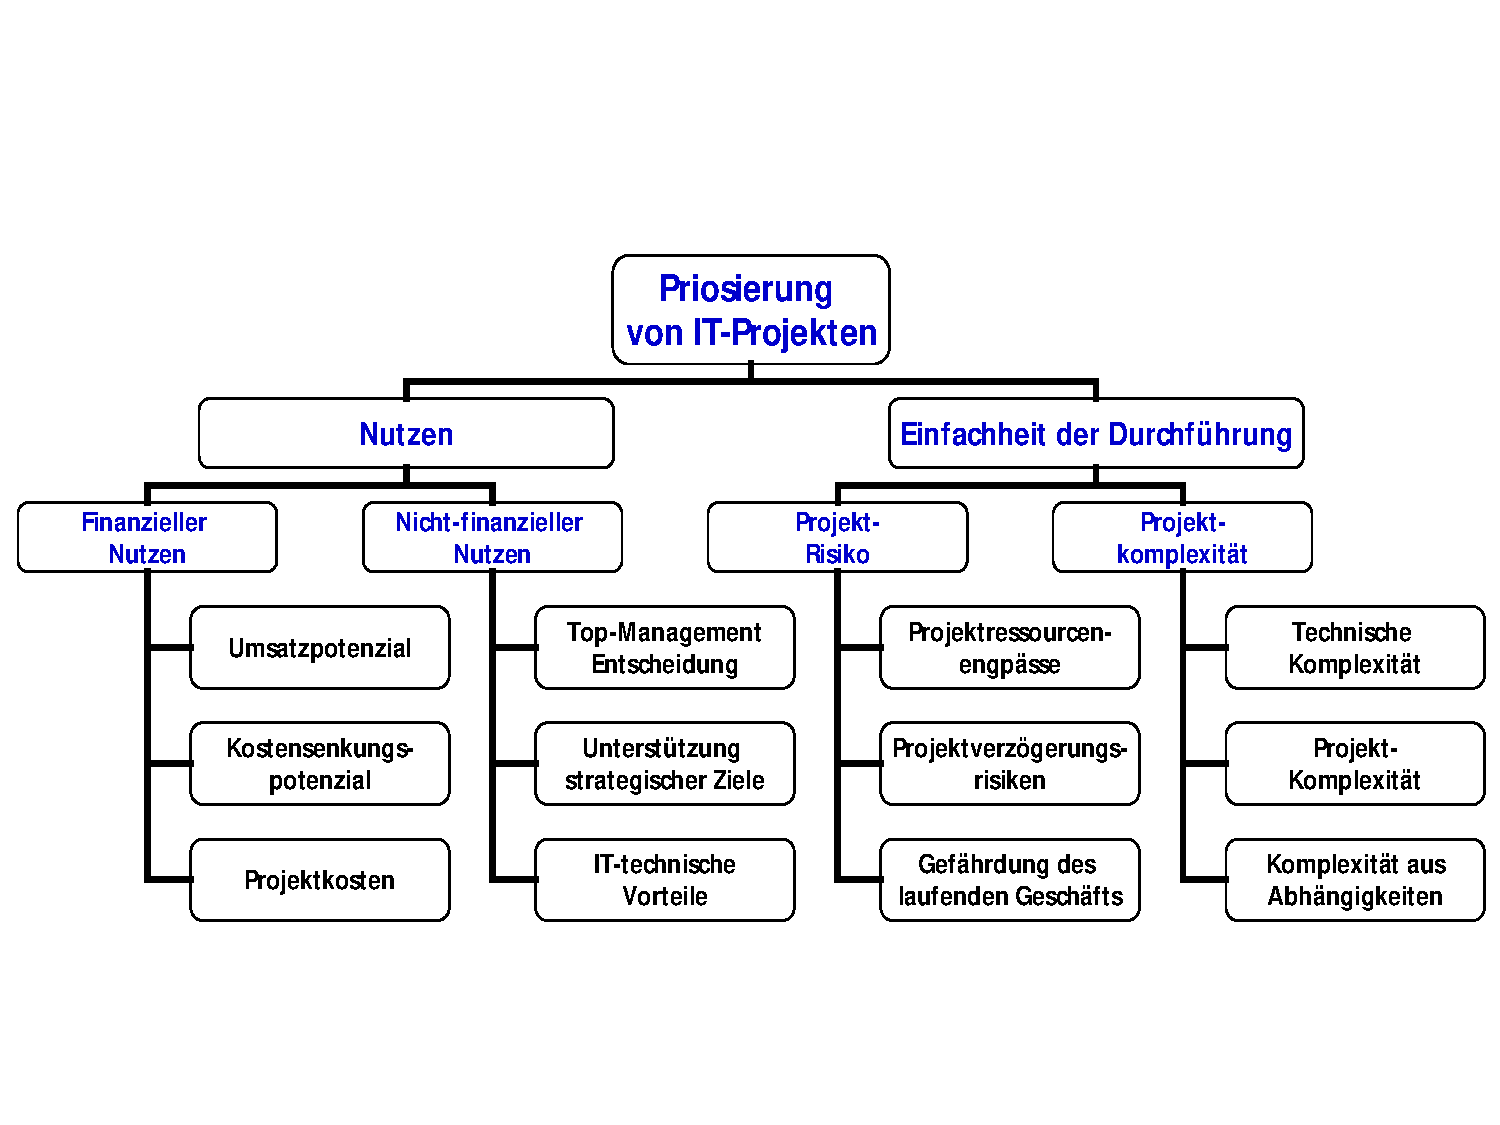
\includegraphics[width=\linewidth]{fig/bewertung-it-projekt}
\caption{Bewertungskriterien von IT-Projekten}
\label{fig:bewertung-it-projekt}
\end{figure}

\section{Nennen Sie Beispiele für typische Fehler im PPM.}

\begin{enumerate}
	\item PPM ist nicht an die Bedürfnisse des Unternehmens angepasst und ist nicht akzeptiert
	\item Zu schwerfällige Prozesse verhindern Innovation
	\item Projektberichte führen nicht zu Entscheidungen
	\item Kein Abbruch von scheiternden Projekten (Abbruch schafft Ressourcen für starke Projekte)
	\item Fehlerhafte Projektdaten (Schätzungen verbessern durch Abgleich mit Ergebnissen)
	\item Keine rechtzeitige Anpassungen der Projektziele
	\item Keine Bereitstellung der benötigten Ressourcen (Genehmigte Projekt müssen ihre Ressourcen kriegen)
	\item Unzureichende Projektplanung
\end{enumerate}

\section{Nennen Sie Beispiele für Standards, die zur Definition eines Unternehmens PPM konsultiert werden können.}

\begin{description}
	\item[IT Infrastructure Library (ITIL):] Gute Quelle für Metriken und Verständnis von Best Practices für IT Strukturen und Prozesse.
	\item[Control Objectives for Information and related Technology (COBIT):] Controlling-Instrumentarium im Rahmen der ITGovernance. 
	\item ISO 38500 (Norm für IT Governance)
\end{description}